\documentclass[10pt]{article} 

\usepackage{booktabs}  % Needed for tables.
\usepackage{graphicx}  % Needed for figures.

\title{A Report}

\date{}

\begin{document}

\maketitle 

% Uid: 1542973251.12672
% Created: 11:40:51 11/23/18 GMT
% Exported: 11:40:51 11/23/18 GMT
% Title: a_report
% Notebook: ../../../README.ipynb
% Data file: ../data/README.ipynb/SalesByRepTable.csv
\providecommand{\SalesByRepTable}{
dummy}
\renewcommand{\SalesByRepTable}{
    \begin{table}[h]
        \centering
        \begin{tabular}{lr}
			\toprule
			{} &    Total \\
			Rep      &          \\
			\midrule
			Andrews  &   149.25 \\
			Gill     &   539.73 \\
			Howard   &    57.71 \\
			Jardine  &   628.74 \\
			Jones    &  1202.50 \\
			Kivell   &   999.50 \\
			Morgan   &   449.10 \\
			Parent   &  1619.19 \\
			Sorvino  &   167.44 \\
			Thompson &    63.68 \\
			\bottomrule
			\end{tabular}

        \caption{Sales totals by sales representative (\$US).}
        \label{SalesByRepTable}
    \end{table}
}


% Uid: 1542973251.469218
% Created: 11:40:51 11/23/18 GMT
% Exported: 11:40:51 11/23/18 GMT
% Title: a_report
% Notebook: ../../../README.ipynb
% Image file: ../figs/README.ipynb/SalesByRepBarChart.pdf
% Data file: ../data/README.ipynb/SalesByRepBarChart.csv
\providecommand{\SalesByRepBarChart}{
dummy}
\renewcommand{\SalesByRepBarChart}{
    \begin{figure}
        \center
        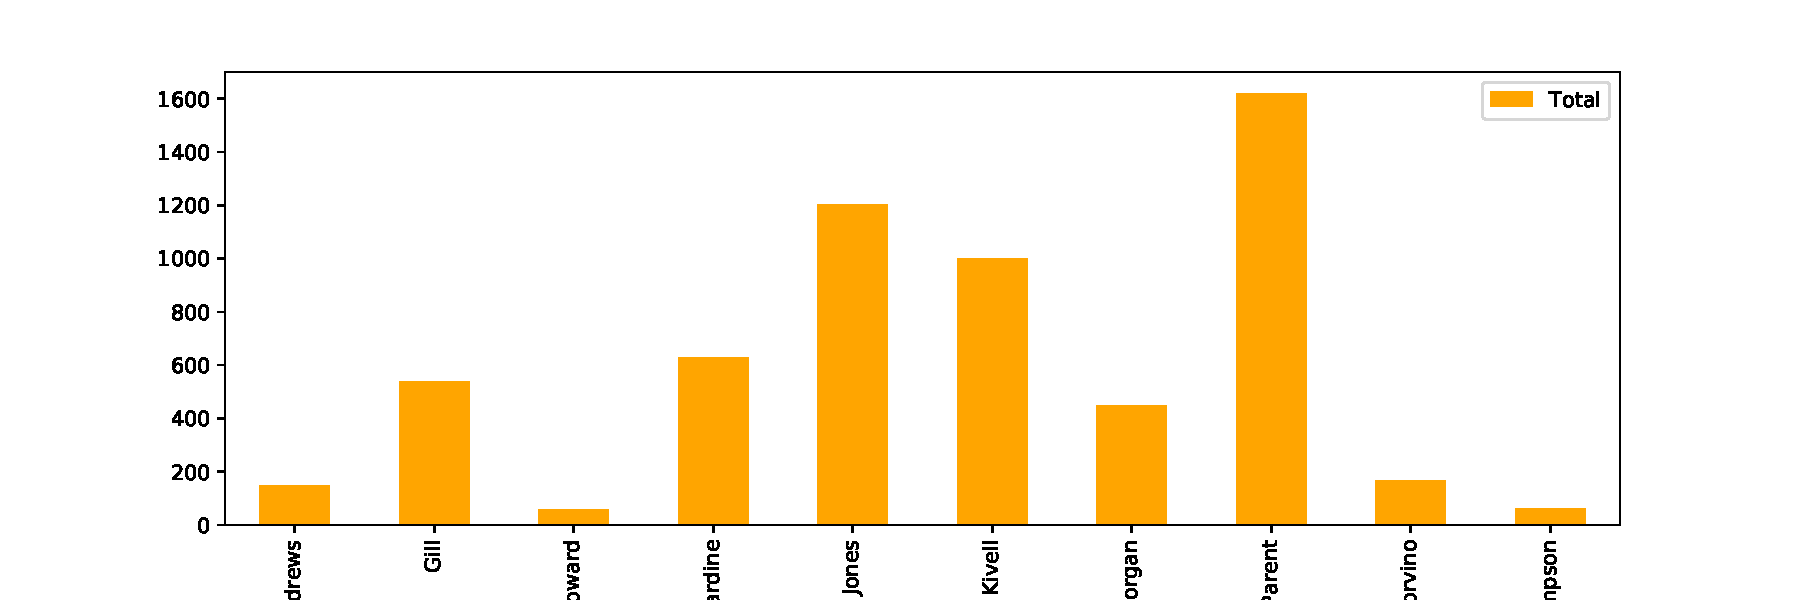
\includegraphics[width=1\textwidth]{../figs/README.ipynb/SalesByRepBarChart.pdf}
        \caption{Sales totals by sales representative (\$US).}
        \label{SalesByRepBarChart}
    \end{figure}
}


% Uid: 1542973252.157745
% Created: 11:40:52 11/23/18 GMT
% Exported: 11:40:52 11/23/18 GMT
% Title: a_report
% Notebook: README.ipynb
\providecommand{\TotalSales}{
dummy}
\renewcommand{\TotalSales}{
5876.84}


% Uid: 1542973254.8277519
% Created: 11:40:54 11/23/18 GMT
% Exported: 11:40:54 11/23/18 GMT
% Title: a_report
% Notebook: ../../../README.ipynb
% Data file: ../data/README.ipynb/SalesByRepTable.csv
\providecommand{\SalesByRepTable}{
dummy}
\renewcommand{\SalesByRepTable}{
    \begin{table}[h]
        \centering
        \begin{tabular}{lr}
			\toprule
			{} &    Total \\
			Rep      &          \\
			\midrule
			Andrews  &   186.56 \\
			Gill     &   674.66 \\
			Howard   &    72.14 \\
			Jardine  &   785.92 \\
			Jones    &  1503.12 \\
			Kivell   &  1249.38 \\
			Morgan   &   561.38 \\
			Parent   &  2023.99 \\
			Sorvino  &   209.30 \\
			Thompson &    79.60 \\
			\bottomrule
			\end{tabular}

        \caption{Sales totals by sales representative (\$AUS).}
        \label{SalesByRepTable}
    \end{table}
}


% Uid: 1542973254.921008
% Created: 11:40:54 11/23/18 GMT
% Exported: 11:40:54 11/23/18 GMT
% Title: a_report
% Notebook: ../../../README.ipynb
% Image file: ../figs/README.ipynb/SalesByRepBarChart.pdf
% Data file: ../data/README.ipynb/SalesByRepBarChart.csv
\providecommand{\SalesByRepBarChart}{
dummy}
\renewcommand{\SalesByRepBarChart}{
    \begin{figure}
        \center
        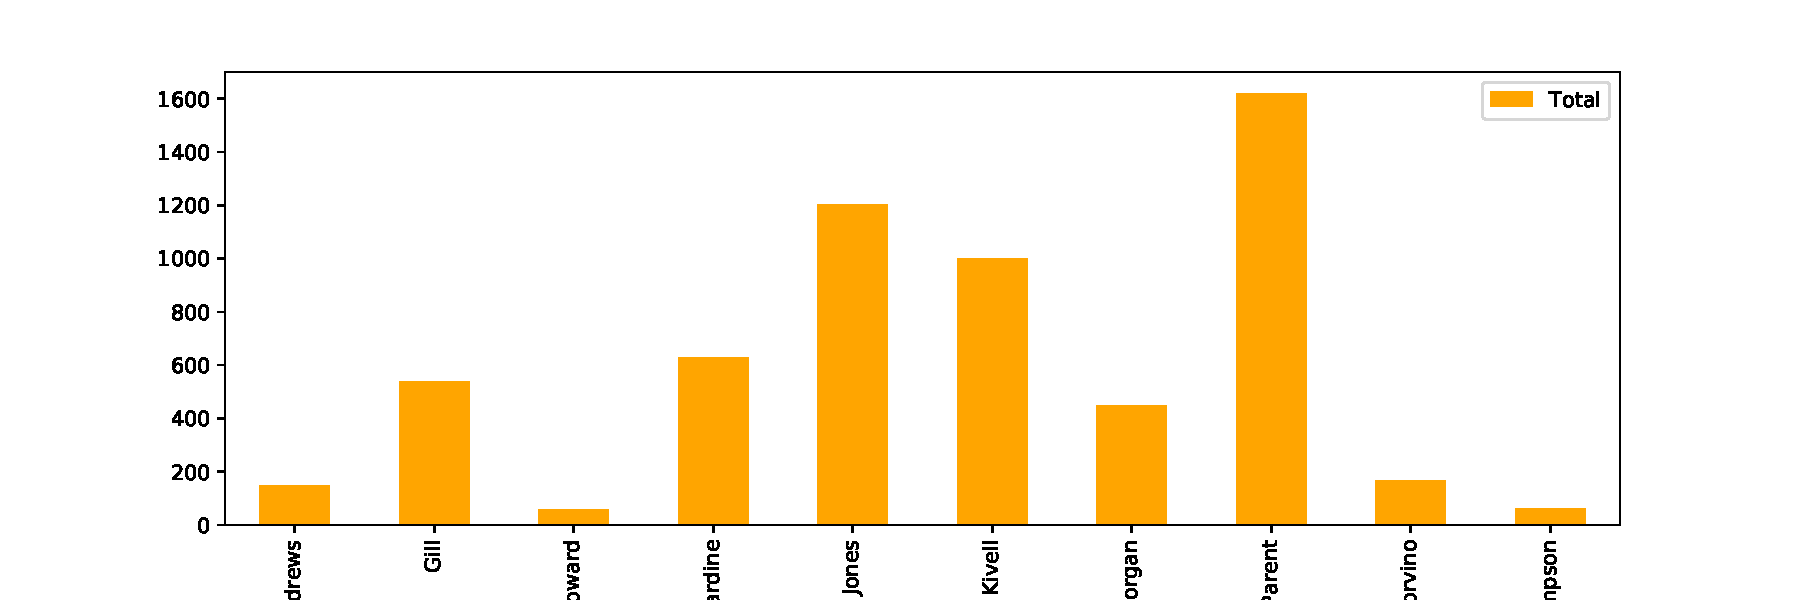
\includegraphics[width=1\textwidth]{../figs/README.ipynb/SalesByRepBarChart.pdf}
        \caption{Sales totals by sales representative (\$AUS).}
        \label{SalesByRepBarChart}
    \end{figure}
}


% Uid: 1542973255.0083652
% Created: 11:40:55 11/23/18 GMT
% Exported: 11:40:55 11/23/18 GMT
% Title: a_report
% Notebook: README.ipynb
\providecommand{\TotalSales}{
dummy}
\renewcommand{\TotalSales}{
7346.05}



   % Include Kallysto defs.

% The text below makes reference to the three 
% exports made from the sample notebook.

Table \ref{SalesByRepTable} summarises the sales totals by sales rep and the same data is also shown in Figure \ref{SalesByRepBarChart}, for an overall sales total of \TotalSales. Notice how the table and figure references in this paragraph are also dynamically created using references to the appropriate export names.

\SalesByRepTable

\SalesByRepBarChart

\end{document}
